\subsection{Business Rules} \label{subsec:BusinessRules}

% TODO: Parameterize business rules

Anybody can challenge anyone else in the Pleistocene Petting Zoo's non-public areas by providing the name of a book and a word contained within the book, and the person being challenged must respond with another word from that book, based on certain rules:
\begin{itemize}
    \item All of the book's words are sorted alphabetically without regard to capitalization (for example, ``hello'' occurs after ``Hear'' and before ``HELP'')
    \item The challenge word occurs \textit{occurrences} times in the book
    \item If $occurrences$ is an even number then the response word is the word is $occurrences$ places \textbf{after} the challenge word in the alphabetized list;
    if the challenge word is less than $occurrences$ places from the start of the list then the response word is the first word in the list
    \item If $occurrences$ is an odd number then the response word is the word $occurrences$ places \textbf{before} the challenge word in the alphabetized list;
    if the challenge word is less than $occurrences$ places from the end of the list then the response word is the last word in the list
\end{itemize}

Here is a simple example.
Suppose the words in the specified book are:

\begin{center}
    \begin{tabular}{cc}
        \textit{word} & \textit{occurrences} \\ \hline
        apple       & 7 \\
        banana      & 4 \\
        carrot      & 15 \\
        date        & 3 \\
        eggplant    & 2 \\
        fig         & 6 \\
        granola     & 9 \\
        horseradish & 9 \\
        ice         & 6 \\
        jelly       & 3 \\
        kale        & 1 \\
        lemon       & 2 \\
        mango       & 8 \\
        naan        & 7 \\
        orange      & 5 \\
        pineapple   & 1 \\
        quinoa      & 11 \\
        raisin      & 4 \\
        spaghetti   & 10 \\
        tomato      & 12 \\
    \end{tabular}
\end{center}
If the challenge word is ``horseradish'' then because horseradish occurs 9 times in the book, the response word is ``quinoa,'' which is 9 places in the list after ``horseradish.''
If the challenge word is ``eggplant'' then the response is ``carrot,'' which is 2 places earlier in the list than ``eggplant.''
If the challenge word is ``quinoa'' then the response word is ``tomato,'' because the response word should be 11 places after ``quinoa,'' but the end of the list is 3 places later;
``tomato'' is the last word in the list.
%(\textit{Note:} ``horseradish'' and ``quinoa'' being each other's response words is coincidental.
%Unusual things happen with short lists of words that do not generalize to longer lists.)

You break the problem down into four sub-problems:

\begin{enumerate}
    \item Designing the Data Structure and Its Algorithms
    \item Alphabetizing Words
    \item Inserting Words
    \item Responding to a Challenge
\end{enumerate}

\subsubsection*{The Books}

Four small ``books'' are included with the starter code:

\begin{itemize}
    \item ``Animals'' (sorted, 7 words)
    \item ``Plants'' (unsorted, 7 words)
    \item ``Cars'' (sorted, 74 words)
    \item ``Food'' (unsorted, 125 words)
\end{itemize}

Two real books have also been reduced to one word per line:\footnote{The text for these books was obtained from \href{https://www.gutenberg.org/}{Project Gutenberg}.
In accordance with Paragraph~1.C of the \href{https://www.gutenberg.org/policy/license}{Project Gutenberg License}, all references to Project Gutenberg have been removed from the ``derived works'' that we are distributing.
    (Removing the references to Project Gutenberg was also necessary to ensure that \textit{only} the words from the books are used for the challenge-and-response system.)}

\begin{itemize}
    \item Mary Shelly's \textit{Frankenstein; Or, The Modern Prometheus} (filename ``Frankenstein'') \url{https://www.gutenberg.org/ebooks/84} (sorted, 74,363 words)
    \item Arthur Conan Doyle's \textit{The Lost World} (filename ``TheLostWorld'')
    \url{https://www.gutenberg.org/ebooks/139} (unsorted, 77,268 words)
\end{itemize}

The very small files of 7 words can be useful for debugging, and the moderate-sized files of 74--125 words should give you confidence in the correctness of your solution.
The real books of more than 74,000 words will be useful to reveal whether you have any memory leaks in your code.
The files marked as \textit{sorted} have all of their words already in alphabetically sorted order, ignoring capitalization;
the files marked as \textit{unsorted} do not have their words sorted (the words in ``Plants'' and ``Food'' are in a randomly-selected order;
the words in ``TheLostWorld'' appear in the order that they appear in the original \textit{The Lost World}).

Each book file, ``\textit{file}'', has a corresponding ``\textit{file}-table.md'' that contains a Markdown-formatted table of the challenge words, the number of occurrences for each challenge word, and the corresponding response word.
You may use these files to confirm the correctness of your solution.

% TODO: re-generate the solution tables

Throughout the assignment, we note that if building the list takes more than a few seconds, there is a bug in your code;
for context, we can build the list for \textit{Frankenstein} in 1--2 seconds and the list for \textit{The Lost World} in 1.5--3 seconds.
We can locate a word (or determine the absence of a word) in the \textit{Frankenstein} list in under 0.5ms and in the \textit{The Lost World} list in under 0.9ms.
Your code may take longer, but it should not take much longer.

% TODO: re-time the sample solution
% TODO: add time-out code to driver

You will earn most of the credit for this lab if your code works for pre-sorted files of up to 200 words.
The remaining credit is for making your code work with unsorted files and, when using files of up to 80,000 words, your code can generate a list and find a word in fewer than 20 seconds.

\vspace{1cm}

H.Awk provides you with the code he worked on.
It turns out that while he finished implemented the array-backed list, he didn't finish the actual challenge-response app.
You decide to warm up by finishing the app and then circling back to the linked list.

\subsection{Word Entries}

The \lstinline{word_entry_t} type is defined in \textit{word\_entry.h}:

\lstinputlisting[linerange=28-31, firstnumber=28]{../starter-code/word_entry.h}

You see that there are also a handful of function prototypes in \textit{word\_entry.h} that would nicely encapsulate this datatype.

\subsubsection{Creating and Destroying Word Entries}

The \function{create_word_entry()} function allocates space for a \lstinline{word_entry_t}, and the \function{delete_word_entry()} function releases that memory.
The \function{create_word_entry()} function, however, does not yet initialize the word entry.

\begin{description}
    \checkoffitem{In \function{create_word_entry()}'s \lstinline{else} block, copy \lstinline{word} into \lstinline{word_entry}'s \lstinline{word} field.}
    \checkoffitem{In \function{create_word_entry()}'s \lstinline{else} block, set \lstinline{word_entry}'s \lstinline{occurrences} field to 0.}
\end{description}

When you copy the word, you must actually copy the word and not merely copy the pointer, for two reasons.
The first reason, from a program design perspective, is that you don't know whether the caller might later put a different word in the array that the \lstinline{word} parameter is in, or the caller might even deallocate that array's memory.
The second reason, from a memory perspective, is that an array embedded in a \lstinline{struct} (such as \lstinline{word_entry_t}'s \lstinline{word} field) is effectively a constant pointer and cannot be re-assigned.

You do not need to make any changes to \function{delete_word_entry()}.

\subsubsection{Accessors and Mutators \\ \footnotesize{\textit{aka}, Getters and Setters}}

We want to control the possible changes that other code might make to a word entry.
Indeed, the only reasonable change would be to increase the number of times that the word is found in a book, whenever we encounter that word again.
Similarly, we want to make sure that data that our ``getter'' functions cannot be used by the caller to make changes to the structure's data.
The \function{get_count()} function returns a value, so there's no hazard there.
The \function{get_word()} function returns a pointer to a constant -- while it \textit{is} possible to discard a \lstinline{const} qualifier, doing so will result in a warning that it will result in undefined behavior.
(The array that the pointer points to isn't actually constant, but the caller is obligated to act as though it is.)

\begin{description}
    \checkoffitem{In \function{increment_count()}, increase the word entry's number of occurrences by one.}
    \checkoffitem{In \function{get_count()}, return the number of occurrences.}
    \checkoffitem{In \function{get_word()}, return a pointer to the word entry's word. (Do \textit{not} make a copy of the word.)}
\end{description}

When returning the word entry's word, simply returning the pointer is sufficient -- and desirable.
It is sufficient because the caller is obligated to treat it as a constant.
The alternative, making a copy, is not desirable because the function doesn't expect the caller to provide a destination, which means that the function would have to allocate memory for the destination;
the caller would be unable to later free this memory without discarding the \lstinline{const} qualifier.

\paragraph{Testing Your Changes}

You can build an executable that uses H.Awk's array-backed list with the command \\
\verb+make arraylistlab+ \\
or, if you want to limit each \function{malloc()} call to no more than 32KB, then use the command \\
\verb+make arraylistlab "OPTION=-DHOBBLE"+

\begin{description}
    \checkoffitem{Build and run the executable.         \\
        \texttt{0) Quit                                 \\
                1) Test word\_entry                     \\
                2) Test list                            \\
                3) Test alphabetical functions          \\
                4) Test insert\_word (empty list)       \\
                5) Test insert\_word (populated list)   \\
                6) Create and print book list           \\
                7) Test challenge/response system       \\
                Select the task you wish to check:}}
    \checkoffitem{Select task 1, ``Test word\_entry''.  \\
        \texttt{0) Return to main menu                  \\
                1) create\_word\_entry()                \\
                2) delete\_word\_entry()                \\
                3) increment\_count()                   \\
                4) get\_count()                         \\
                5) get\_word()                          \\
                Select the function you wish to check:}}
    \checkoffitem{Select function 1, ``create\_word\_entry()'', and enter a word when prompted.}
\end{description}

The word entry will be displayed.
For example, if your word was ``foo'' then the output will be: \\
\texttt{Created --           0 : foo}

\begin{description}
    \checkoffitem{Use fuctions 3 (``increment\_count()''), 4 (``get\_count()''), and 5 (``get\_word()'') to test your code.}
    \checkoffitem{Continue to test until you discover a bug or are satisfied that your implementations are correct.}
    \checkoffitem{When you have finished, use function 2 (``delete\_word\_entry()'') to release the word entry's memory, then select 0 to return to the main menu, and then select 0 to exit the program.}
    \begin{itemize}
        \item Note: whenever you return to the main menu, any existing list will be deleted.
            No memory references survive when moving between one main-menu-option and another.
    \end{itemize}
\end{description}



\subsection{Alphabetical Functions}

\subsubsection{Making a Lowercase Copy of a Word}

Because the book's words should be insensitive to capitalization, we will store the words with all of their letters in lowercase.
In \textit{challenge-response.c}, there is a \function{word_to_lowercase()} function to do just that.

\begin{description}
    \checkoffitem{Implement the \function{word_to_lowercase()} function.}
\end{description}

Unlike keyboardlab, you can use the \function{tolower()} function\footnote{\url{https://en.cppreference.com/w/c/string/byte/tolower}} from \texttt{ctype.h}.

\subsubsection{Comparing Words}

Because the book's words need to be sorted, we need to be able to compare words.
In \textit{challenge-response.c}, there are three functions to do that:
\begin{description}
    \item[words\_are\_equal()] which returns \lstinline{true} if and only if the two words are indistinguishable
    \item[word1\_is\_earlier\_than\_word2()] which returns \lstinline{true} if and only if the first word precedes the second word in an alphabetically-sorted list
    \item[word1\_is\_later\_than\_word2()] which returns \lstinline{true} if and only if the first word follows the second word in an alphabetically-sorted list
\end{description}

\begin{description}
    \checkoffitem{Implement the \function{words_are_equal()} function.}
    \checkoffitem{Implement the \function{word1_is_earlier_than_word2()} function.}
    \checkoffitem{Implement the \function{word1_is_later_than_word2()} function.}
\end{description}

We recommend that you use the \function{strncmp()} function\footnote{\url{https://en.cppreference.com/w/c/string/byte/strncmp}} from \texttt{string.h}.

\paragraph{Testing Your Changes}

You can build an executable that uses H.Awk's array-backed list with the command \\
\verb+make arraylistlab+ \\
or, if you want to limit each \function{malloc()} call to no more than 32KB, then use the command \\
\verb+make arraylistlab "OPTION=-DHOBBLE"+

\begin{description}
    \checkoffitem{Build and run the executable.         \\
        \texttt{0) Quit                                 \\
                1) Test word\_entry                     \\
                2) Test list                            \\
                3) Test alphabetical functions          \\
                4) Test insert\_word (empty list)       \\
                5) Test insert\_word (populated list)   \\
                6) Create and print book list           \\
                7) Test challenge/response system       \\
                Select the task you wish to check:}}
    \checkoffitem{Select task 3, ``Test alphabetical functions'', and enter words when prompted.}
\end{description}

Each word will be displayed in its lowercase form, and the results of the three comparison functions will be shown.

\begin{description}
    \checkoffitem{Continue to test until you discover a bug or are satisfied that your implementations are correct.}
    \checkoffitem{When you have finished, select 0 to exit the program.}
\end{description}


\subsection{Preparing to Work with Lists}

It is entirely probably that H.Awk, left to his own devices, would simply have used an array instead of making the effort to create an array-backed list with a well-defined abstract model.
Fortunately, someone pulled his strings, and you have available to you an abstract model of a list that can be realized by any number of implementations.

Like \lstinline{word_entry_t}, the \lstinline{list_t} datatype has functions to encapsulate it.
In the case of \lstinline{list_t}, however, this encapsulation is essential because the code in \textit{challenge-response.c} has access to the type declaration but not the type definition.

\begin{description}
    \checkoffitem{Review the datatype and functions declared in \textit{list.h}.}
\end{description}

A list is abstractly modeled as having a sequence of word entries and an iterator that points to the ``current'' word entry.
The iterator can point to anywhere between the first word entry to the ``empty'' space after the last word entry.

The \function{reset_iterator()} function sets the iterator to the first word entry, and the \function{iterate_forward()} and \function{iterate_backward()} functions cause the iterator to advance and retreat.
These functions return \lstinline{true} if successful, and \lstinline{false} if not.
``Not successful'' isn't a bad thing, though -- the implications are informative:
\begin{itemize}
    \item \lstinline{reset_iterator()} fails only when there is no first element; that is, when the list is empty
    \item \lstinline{iterate_forward()} fails only when iterating forward is not possible; that is, when the iterator already points to the ``empty'' space after the last word entry
    \item \lstinline{iterator_backward()} fails only when iterating backward is not possible; that is, when the iterator already points to the first word entry
\end{itemize}

The \function{get_word_entry()} function retrieves the word entry that the iterator points to.
The \function{insert()} function inserts the word entry before the word entry that the iterator currently points to.
And the \function{delete()} function removes the word entry that the iterator currently points to.

There are three functions that do not depend on the iterator:
\function{get_first_word_entry()} and \function{get_last_word_entry()}, with the obvious meanings,
and \function{append()} that places a word entry at the end of the sequence.

\begin{description}
    \checkoffitem{Review the \function{respond()} function in \textit{challenge-response.c} to see some uses of the \lstinline{list_t} functions.}
\end{description}


\subsection{Inserting Words}

The \function{build_list()} function in \textit{challenge-response.c} reads words from a ``book'' and sends them to \function{insert_word()}.
You do not need to implement \function{build_list()}.

The \function{insert_word()} function in \textit{challenge-response.c} finds the correct place in the list for a lowercase copy of the word.
If the word is already in the list, then it increments the word's count;
otherwise, it inserts the word into the list.
You will implement \function{insert_word()}.

\subsubsection{Limited Implementation}

The simplest implementation of \function{insert_word()} is to assume that the words in the book are already sorted -- as they are for ``Animals'', ``Cars'', and ``Frankenstein''.
In this case, you know that if the word is already in the list then it is the last word in the list,
and if the word is not already in the list then it belongs at the end of the list.

You will receive half of the credit for \function{insert_word()} if it works on pre-sorted books.
If you choose to use this implementation:
\begin{description}
    \checkoffitem{Implement \function{insert_word()} for pre-sorted books}
    \checkoffitem{Test this implementation and move on to implementing a linked list}
    \checkoffitem{Return to this sub-problem later to attempt a more-general implementation}
\end{description}

Otherwise, implement Insertion Sort\dots

\subsubsection{Insertion Sort}

While you probably learned about sorting in \cstwo, you may not have learned about \textit{Insertion Sort}.
If you did learn about Insertion Sort, you probably learned to use it to sort an array or list in-place, and that it's a $\mathcal{O}(n^2)$ algorithm that is less efficient than $\mathcal{O}(n \log n)$ sorting algorithms such as Merge Sort and Quick Sort.
Insertion Sort is often taught as a way to sort an array in-place,
but a variation of Insertion Sort has a particular advantage in that it can be applied \textit{as the list is built}, making for a much simpler and less error-prone implementation than a different sort that requires the list to already be built.

Your Insertion Sort algorithm will read an input and then traverse a sorted list to find the proper location in the sorted list for the input.
The input is then inserted into the list at that location, preserving the property that the list is sorted.

\begin{description}
    \checkoffitem{Implement \function{insert_word()} such that:}
        \begin{itemize}
            \item The function looks for the word in the sorted list
            \item If the word is found in its proper location in the sorted list, then update the number of occurrences
            \item If the word is not present in its proper location in the sorted list, then insert a new node for that word at its proper location
        \end{itemize}
\end{description}

\paragraph{Testing Your Changes}

If you were to apply category-partition testing, you might arrive at these categories and partitions:

\begin{center} \begin{tabular}{c|c}
    \textbf{Categories}             & \textbf{Partitions}                   \\ \hline\hline
    Word's position in the list     & only word in the list                 \\
                                    & at the start of the list              \\
                                    & at the end of the list                \\
                                    & somewhere in the middle of the list   \\ \hline
    Word is already in the list?    & yes                                   \\
                                    & no                                    \\ \hline
    Word is already lowercase?      & yes                                   \\
                                    & no
\end{tabular}\end{center}

\begin{description}
    \checkoffitem{Build and run the executable.         \\
        \texttt{0) Quit                                 \\
                1) Test word\_entry                     \\
                2) Test list                            \\
                3) Test alphabetical functions          \\
                4) Test insert\_word (empty list)       \\
                5) Test insert\_word (populated list)   \\
                6) Create and print book list           \\
                7) Test challenge/response system       \\
                Select the task you wish to check:}}
\end{description}

You can test ``only word in the list''/``word is not already in the list'' with task 4.
You can test most of the other combinations with task 5.\footnote{The only combination not supported is ``only word in the list''/``word is already in the list'' -- but testing ``at the start of the list''/``word is already in the list'' and/or ``at the end of the list''/``word is already in the list'' should exercise the code that would be used by ``only word in the list''/``word is already in the list,''}
When you select these options, an initial sorted list (empty or pre-populated, as appropriate) will be created and printed, and you will be prompted to enter a word.
After you have entered a word, \function{insert_word()} will be called, and the resulting sorted list (with a new word with 1 occurrence, or with an existing word's occurrences increased by 1) will be printed.

\begin{description}
    \checkoffitem{Test \function{insert_word()} until you discover a bug or are satisfied that your implementation is correct.}
\end{description}


\subsection{Testing the Challenge-Response System} \label{subsec:TestingChallengeResponse}

When you are satisfied that your word entry, alphabetical, and word insertion functions are correct, test their integration into the challenge-response system.
With task 6, you will be prompted for the name of a book file, and then the list will be generated and printed.
With task 7, you will be prompted for the name of a book file, and then the list will be generated; you will then be repeatedly prompted for challenge words which will produce responses.
You can use the ``\textit{file}-table.md'' files to confirm the correctness of the results.

\textcolor{red}{If your program requires more than a few seconds to build a list, or does not get a challenge word's response nearly instantaneously, then there is a bug in your code.}

\begin{description}
    \checkoffitem{Test building a list until you discover a bug or are satisfied that your implementations are correct.}
    \checkoffitem{Test challenge/responses until you discover a bug or are satisfied that your implementations are correct.}
    \checkoffitem{When you have finished, select 0 to exit the program.}
\end{description}

As a reminder, the book files are:

\begin{itemize}
    \item ``Animals'' (sorted, 7 words)
    \item ``Plants'' (unsorted, 7 words)
    \item ``Cars'' (sorted, 74 words)
    \item ``Food'' (unsorted, 125 words)
    \item ``Frankenstein'' (sorted, 74,363 words)
    \item ``TheLostWorld'' (unsorted, 77,268 words)
\end{itemize}


\subsection{Linked List} \label{subsec:LinkedList}

\textit{n.b.}: If you need a refresher on linked lists, see Appendix~\ref{sec:linkedLists}.

In \textit{list.h}, we use a forward declaration to make the code in \textit{challenge-response.h} aware of the type.

\lstinputlisting[linerange=46-46, firstnumber=46]{../starter-code/list.h}

When you built the \textit{arraylistlab} executable earlier, the \textit{array\_list.h} file provided a type definition for the code in \textit{array\_list.c} to use.
Similarly, when you build the \textit{linkedlistlab} executable, the \textit{linked\_list.h} file provided a type definition for the code in \textit{linked\_list.c} to use.

\lstinputlisting[linerange=56-60, firstnumber=56]{../starter-code/linked_list.h}

The list definition has pointers to three nodes, a \lstinline{head} that points to the first node in the list, a \lstinline{tail} that points to the last node in the list, and a \lstinline{current} that serves as the ``iterator'' for the list's abstract model.
\textcolor{red}{
    Some notes about \lstinline{NULL} pointers -- we will adopt the convention that:
    \begin{itemize}
        \item \lstinline{head} and \lstinline{tail} are \lstinline{NULL} if and only if the list is empty
        \item \lstinline{current_node} is \lstinline{NULL} if the iterator points to the ``empty'' space after the last word entry (or the list is empty)
    \end{itemize}
}

We define a linked list note conventionally:

\lstinputlisting[linerange=31-31, firstnumber=31]{../starter-code/linked_list.h}
\dots
\lstinputlisting[linerange=41-45, firstnumber=41]{../starter-code/linked_list.h}

(Here the forward declaration is necessary so that \lstinline{node_t} can be used when defining the node structure.)

When writing functions in \textit{challenge\_response.c}, you had to rely on \lstinline{list_t}'s encapsulation and could not assume any particular list definition.
\textbf{Whenever you are writing a function in \textit{linked\_list.c}, you can treat \lstinline{list_t} as though it has the linked list definition.}


\subsection{Building and Testing Your Linked List Implementation}

If you use the command \\
\verb+make all+ \\
or \\
\verb+make all "OPTION=-DHOBBLE"+ \\
then you will generate two executables: \textit{arraylistlab} that has the array-backed list, and \textit{linkedlistlab} that has the linked list.
If you open two terminal windows, you can run the test code on \textit{arraylistlab} in one window and run the test suite on \textit{linkedlistlab} in the other window.
This will allow you to compare the results with your linked list implementation against the expected results provided by the array-backed list (Figure~\ref{fig:SideBySideTesting}).

\begin{figure}
    \centering
    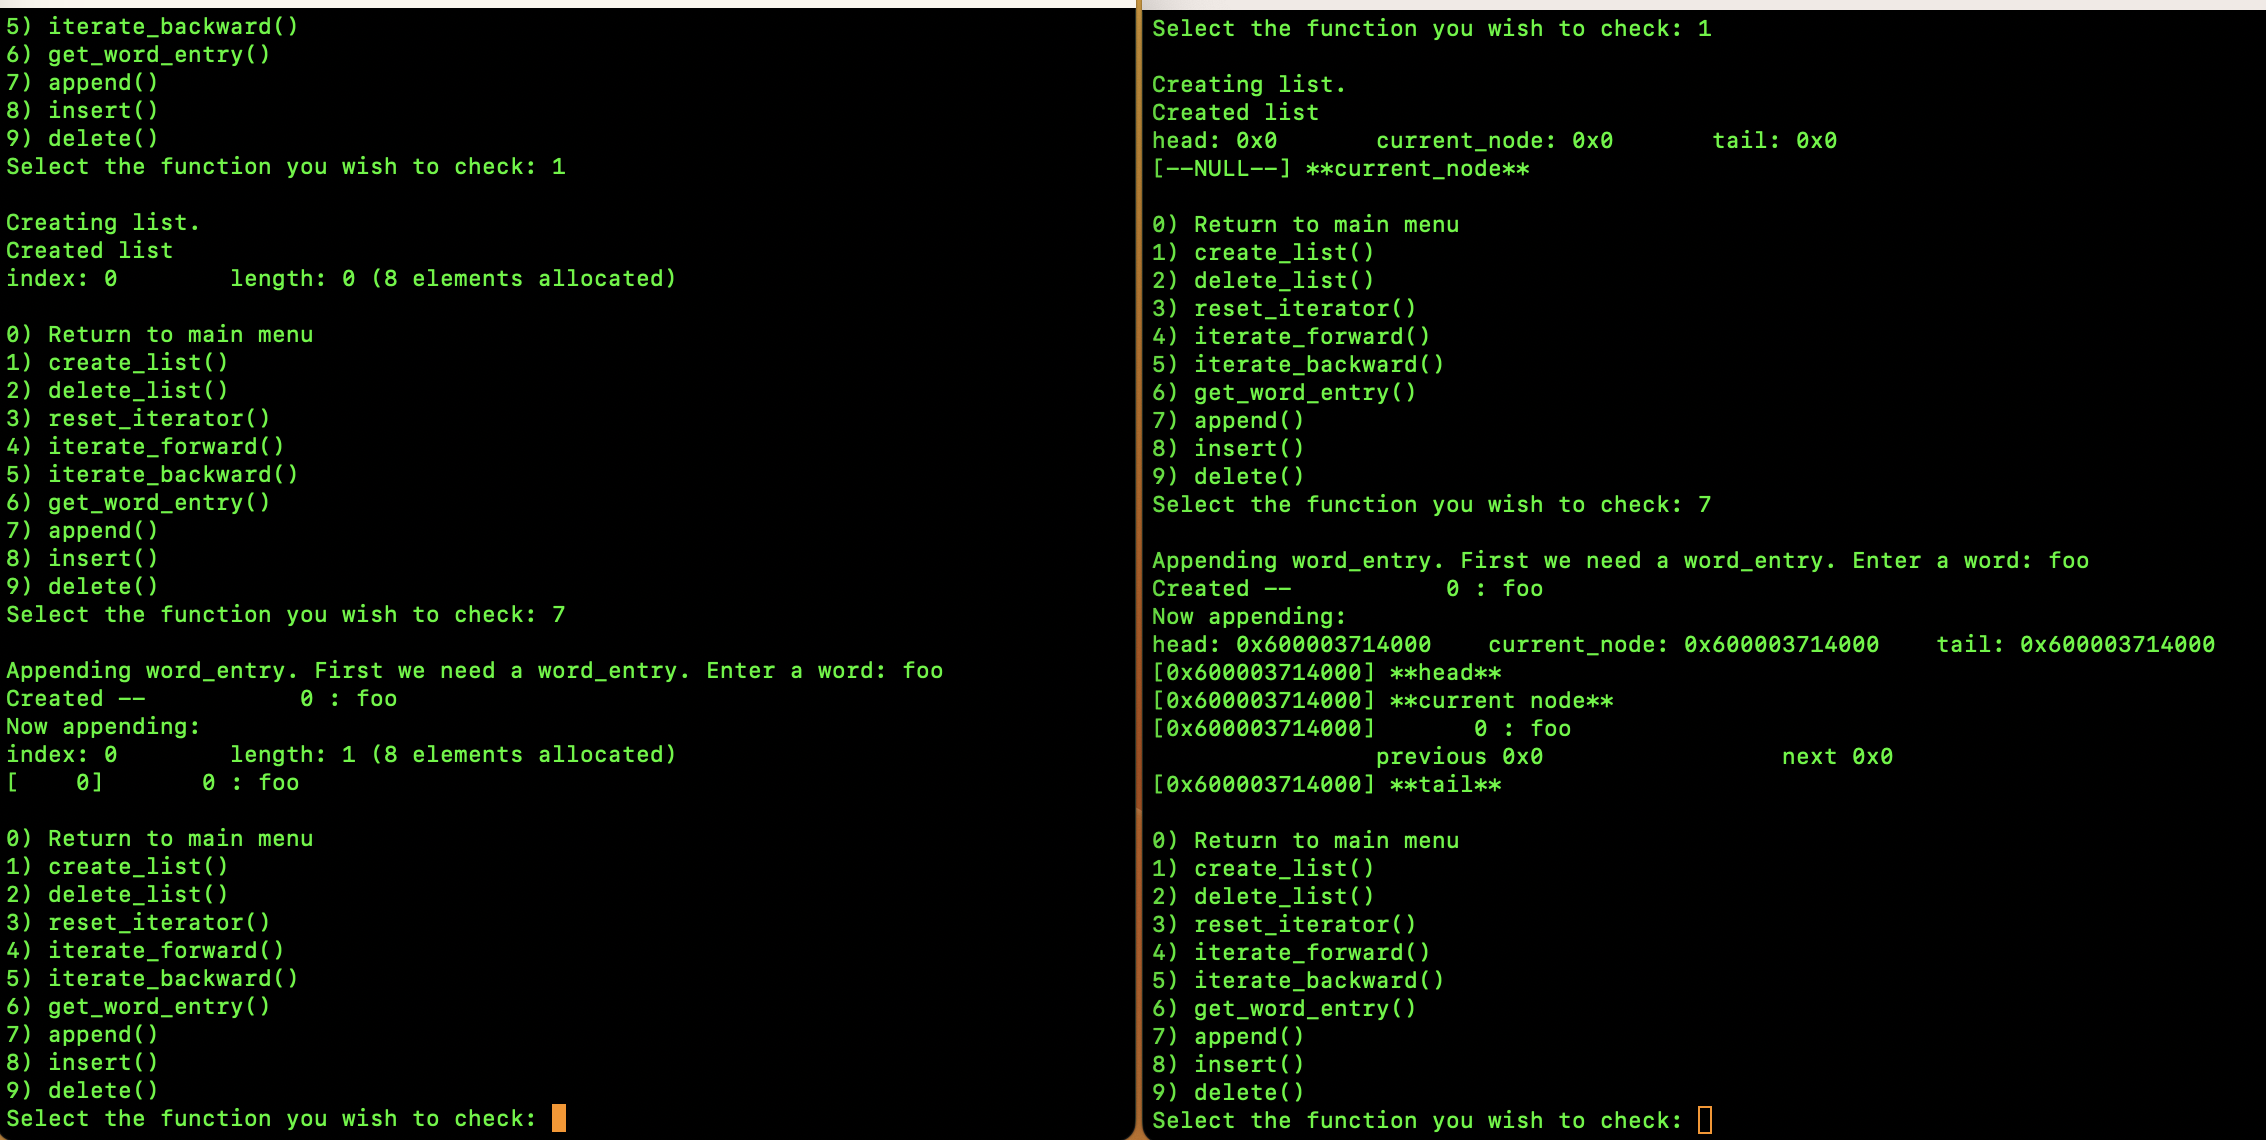
\includegraphics[width=6in]{SideBySideTesting}
    \caption{Testing an array-backed list (left) and a linked list (right) side-by-side.}
    \label{fig:SideBySideTesting}
\end{figure}

To test your linked list implementation, run \textit{linkedlistlab} (and, optionally, \textit{arraylistlab} in another terminal window),
and select option 2, ``Test list''


\subsection{Creating a Node, Creating a List}

In \textit{linked\_list.c}:

\begin{description}
    \checkoffitem{Edit \function{create_node()} to initialize all of a new node's fields.}
    \checkoffitem{Edit \function{create_list()} to initialize all of a new list's fields.}
    \checkoffitem{Test \function{create_node()} and \function{create_list()} by selecting option 2 (``Test list'') and function 1 (``create\_list()'').}
    \checkoffitem{Free the memory by selecting function 2 (``delete\_list()'').
        Exit out of the program by selecting function 0, then option 0.}
\end{description}

It is unlikely that you made any errors that would cause the ``create\_list()'' test to fail,
but it's better to find out now if you did.


\subsection{Appending a Node}

The \function{append()} function takes a word entry, makes it the payload of a new node, and places the new node at the end of the linked list.
The new node, of course, becomes the tail of the list.
If the list is initially empty, then the new node is also the head of the list.

\begin{description}
    \checkoffitem{Edit \function{append()} to place a word entry at the end of the list.}
    \checkoffitem{Create a list by selection option option 2 (``Test list'') and function 1 (``create\_list()'').}
    \checkoffitem{Test \function{append()} for an empty list by selecting function 7 (``append()'').}
    \checkoffitem{Test \function{append()} for a list with one node by selecting function 7 (``append()'').}
    \checkoffitem{Test \function{append()} for a list with multiple nodes by selecting function 7 (``append()'').}
    \checkoffitem{Free the memory by selecting function 2 (``delete\_list()'').
        Exit out of the program by selecting function 0, then option 0.}
\end{description}


\subsection{Iterator Manipulation}

The \function{reset_iterator()} function should make the iterator point to the first element in the sequence.
For a linked list, this means that the current node should be the head.
If successful, then the function returns \lstinline{true},
but if there isn't a first element (that is, if the head is \lstinline{NULL}) then the function returns \lstinline{false}.

The \function{iterate_forward()} and \function{iterate_backward()} functions cause the iterator to move back and forth across the sequence.
For a linked list, this means that you follow the current node's \lstinline{next} or \lstinline{previous} pointers, as appropriate.

\begin{description}
    \checkoffitem{Implement \function{reset_iterator()}.}
    \checkoffitem{Implement \function{iterate_forward()}.}
    \checkoffitem{Implement \function{iterate_backward()}.}
    \checkoffitem{Create a list by selection option option 2 (``Test list'') and function 1 (``create\_list()'').}
    \checkoffitem{Test these functions on an empty list by selecting function 3 (``reset\_iterator()''), function 4 (``iterate\_forward()''), and function 5 (``iterate\_backward()'').
        The test should state that the iterator doesn't change for any of these functions.}
    \checkoffitem{Create a list with one node by selecting function 7 (``append()'').}
    \checkoffitem{Test these functions on a singleton list by selecting function 3 (``reset\_iterator()''), function 4 (``iterate\_forward()''), and function 5 (``iterate\_backward()'').
        Pay attention to whether the test states that the iterator changed or not.
        When the iterator does change, you should also see that the address of the current node has changed.}
    \checkoffitem{Create a list with multiple nodes by selecting function 7 (``append()'').}
    \checkoffitem{Continue to test the iterator manipulation functions until you discover a bug or are satisfied that your implementations are correct.}
    \checkoffitem{Free the memory by selecting function 2 (``delete\_list()'').
        Exit out of the program by selecting function 0, then option 0.}
\end{description}


\subsection{Examining Word Entries}

The \function{get_word_entry()} function retrieves the current node's word entry.
The \function{get_first_word_entry()} and \function{get_last_word_entr()} retrieve the head's and tail's word entries, respectively.
If the current, head, or tail pointers are \lstinline{NULL}, then the corresponding functions return \lstinline{NULL}.

\begin{description}
    \checkoffitem{Implement \function{get_word_entry()}.}
    \checkoffitem{Implement \function{get_first_word_entry()}.}
    \checkoffitem{Implement \function{get_last_word_entry()}.}
    \checkoffitem{Create a list by selection option option 2 (``Test list'') and function 1 (``create\_list()'').}
    \checkoffitem{Test \function{get_word_entry()} on an empty list by selecting function 6 (``get\_word\_entry()'').}
    \checkoffitem{Create a list with one node by selecting function 7 (``append()'').}
    \checkoffitem{Test \function{get_word_entry()} on a singleton list.
        Test it with the iterator pointing at the only node in the list,
        and test it with the iterator pointing at the ```empty'' space after the word entry}
    \checkoffitem{Create a list with multiple nodes by selecting function 7 (``append()'').}
    \checkoffitem{Continue to test \function{get_word_entry()} until you discover a bug or are satisfied that your implementation is correct.}
    \checkoffitem{Free the memory by selecting function 2 (``delete\_list()'').
        Exit out of the program by selecting function 0, then option 0.}
\end{description}


\subsection{Inserting a Node}

The \function{insert()} function takes a word entry, makes it the payload of a new node, and places the new node before the current node and after the current node's predecessor node.
The new node, becomes the current node.
There are a couple of special cases:
\begin{itemize}
    \item If the list is initially empty, then the new node is also the head and the tail of the list.
    \item If the current node is \lstinline{NULL} but there is head and tail, then the iterator points at the ``empty'' space after the last word entry.
        In this case, the new node is also the tail.
\end{itemize}

\begin{description}
    \checkoffitem{Implement \function{insert()}.
        Be sure to handle its special cases.}
    \checkoffitem{Create a list by selection option option 2 (``Test list'') and function 1 (``create\_list()'').}
    \checkoffitem{Test \function{insert()} on an empty list by selecting function 8 (``insert()'').}
    \checkoffitem{Thoroughly test \function{insert()} until you discover a bug or are satisfied that your implementation is correct.
        (Use the iterator manipulation functions to move the iterator to where it needs to be for each test.)}
    \checkoffitem{Free the memory by selecting function 2 (``delete\_list()'').
        Exit out of the program by selecting function 0, then option 0.}
\end{description}


\subsection{Deleting a Node} \label{subsec:DeletingNode}

The \function{delete()} function removes and deletes the current node from the list, updating its neighbors' \lstinline{next} and \lstinline{previous} pointers (and possibly the list's \lstinline{head} or \lstinline{tail} pointer) accordingly.
After the deletion, the deleted node's successor node becomes the current node.
\begin{itemize}
    \item[] \textit{Exception} -- if the deleted node was the list's tail, then that node's ``successor'' is the ``empty'' space after the last word entry.
        In this case, the new tail should become the current node.
    \item[] \textit{Exception to the exception} -- if the deleted node was the only node in the list, then there isn't a new tail, and so the current node is \lstinline{NULL}.
\end{itemize}

\begin{description}
    \checkoffitem{Implement \function{delete()}.
        Be sure to handle its special cases.}
    \checkoffitem{Create a list by selection option option 2 (``Test list'') and function 1 (``create\_list()'').}
    \checkoffitem{Populate the list with several using \function{append()} and/or \function{insert()}.}
    \checkoffitem{Thoroughly test \function{delete()} (function 9) until you discover a bug or are satisfied that your implementation is correct.
        (Use the iterator manipulation functions to move the iterator to where it needs to be for each test.
        Place more word entries in the list if  you need to.)}
    \checkoffitem{Free the memory by selecting function 2 (``delete\_list()'').
    Exit out of the program by selecting function 0, then option 0.}
\end{description}


When you are satisfied that your linked list functions are correct, test their integration into the challenge-response system.
You can use the ``\textit{file}-table.md'' files to confirm the correctness of the results.

\textcolor{red}{If your program requires more than a few seconds to build a list, or does not get a challenge word's response nearly instantaneously, then there is a bug in your code.}

\begin{description}
    \checkoffitem{Test building a list until you discover a bug or are satisfied that your implementations are correct.}
    \checkoffitem{Test challenge/responses until you discover a bug or are satisfied that your implementations are correct.}
    \checkoffitem{When you have finished, select 0 to exit the program.}
\end{description}

As a reminder, the book files are:

\begin{itemize}
    \item ``Animals'' (sorted, 7 words)
    \item ``Plants'' (unsorted, 7 words)
    \item ``Cars'' (sorted, 74 words)
    \item ``Food'' (unsorted, 125 words)
    \item ``Frankenstein'' (sorted, 74,363 words)
    \item ``TheLostWorld'' (unsorted, 77,268 words)
\end{itemize}

Your code might already be able to handle large files in just a few seconds, in which case you are finished.

On the other hand, your code might run briskly when working with smaller files of only a couple of hundred words but then become very sluggish when the number of words is in the thousands.
This tends to be due to one (or both) of two causes.
Look for inefficient algorithms, and look for memory leaks.
If you use the \texttt{top} utility while running your program, and you notice that your program is allocating more than 10MB, then you probably have a memory leak.
If your program is allocating more than 1GB, then your program most certainly has a memory leak.
